%
%	Theorieteil
%

\pagebreak
\section{Infrastructure as Code}

\onehalfspacing

\subsection{Terraform}

All major cloud providers have their infrastructure scripting tools (Azure Resource Manager, AWS Cloud Formation). Still, there's one declarative tool that's available for all infrastructure platforms, on-premise or public: Terraform by HashiCorp.\footnote{See \textit{HashiCorp (2019)}: Deliver infrastructure as code with Terraform. \cite{terraform}}.

As of Rancher 2.3, released in October 2012, Rancher has a stable Terraform provider.\footnote{See \textit{Rancher Labs (2019)}: Introducing the Rancher 2 Terraform Provider. \cite{terraformProvider}} You can easily create and decommission Kubernetes clusters from a Terraform plan as part of a move of Enterprise IT to Infrastructure-as-Code.

With Terraform, creating infrastructure becomes as easy as writing a piece of code. Terraform integrates nicely with your existing source code revision systems, such as GitHub or GitLab. It will also ensure that all infrastructure deployments are repeatable and uniformly executed.

Adding Terraform to the container run-time tool chest of Rancher and Kubernetes is a major benefit and huge step forward, as it will make the creation of new Kubernetes clusters so much easier.\footnote{See \textit{Frank, C. (2020)}: Deploy Kubernetes Clusters on Microsoft Azure with Rancher. \cite{deployAzure}}

\subsection{Templates}

Another essential piece for your Kubernetes tool chest is templates. Templates will allow you to define certain configuration items across the organization, which will help a lot when dealing with hardening in the next chapter. By using templates and establishing policies that make their use mandatory, you can enforce settings and hide some details, such as credentials.

Rancher offers templates on several levels:

\begin{itemize}
\item Cloud Credentials
\item Node Templates
\item Cluster Templates
\end{itemize}

We'll look at each of these in more detail below, but let's first look at the different possibilities of creating a Kubernetes cluster from within Rancher.

\subsection{Kubernetes Cluster Creation}

\subsubsection{Managed Kubernetes}

Overall there are three options to create a Kubernetes cluster with Rancher on any of the big public cloud providers:

\begin{itemize}
\item Managed Kubernetes (GKE, AKS, EKS)
\item Rancher node-driver (Azure, AWS)
\item Custom nodes (GCP, Azure, AWS)
\end{itemize}

To create a managed Kubernetes cluster, you'll have to follow the following steps:

First, within a  Terraform plan, define the Rancher provider. Then, in the Rancher cluster definition, define the GKE, AKS, or EKS options and finally have Terraform create the cluster. Terraform will be using the platform API for this.

In this setup, the cloud provider will manage the Kubernetes control plane, and Rancher's functionality will be a bit more limited than in the next option.

\subsubsection{Rancher Node-Driver}

If you're happy to have Rancher manage the control plane and have full control, and are on either AWS or Azure, consider using the Rancher node-driver. To do this, following the following steps:

First, within a  Terraform plan, define the Rancher provider. Second, in the Rancher cluster definition, define Azure or AWS cloud provider within the RKE cluster options. Then, create the appropriate cloud credentials and node templates. Finally, have Terraform create the cluster, using docker-machine.

Using the Rancher node-driver is the most preferred option and the one that we will follow throughout the document.

\subsubsection{Custom Nodes}

If you need more fine-grained control over the underlying infrastructure, Rancher also offers the ability to use custom created nodes for its Kubernetes clusters. For this, you'll need to follow these steps:

First, within a  Terraform plan, define both the Rancher provider and an infrastructure provider. Second, in the Rancher cluster definition, define the cloud provider within the RKE cluster options. Then, have Terraform create the cluster nodes with the infrastructure provider and pass the Rancher registration command to cloud-init

Although this is the most flexible approach, Rancher will lose the ability to scale the node pools, among other features. It also requires that the Terraform plans have access to credentials for the infrastructure provider, unlike in the option above, where you could provide them centrally in Rancher.

\subsubsection{Import}

A fourth and final option would be to create clusters completely outside of Terraform and Rancher and manually import them into Rancher later. Importing clusters is an entirely valid option, but outside of our document's scope, it would require other forms of automation.

\subsection{Rancher Provider}

Let's start defining our Kubernetes cluster. The first step is to set up the credentials for Rancher. All API access to Rancher is controlled from the built-in RBAC controller, and every user can create their own API keys.

\begin{figure}[H]
\centering
\caption {Rancher API Key}
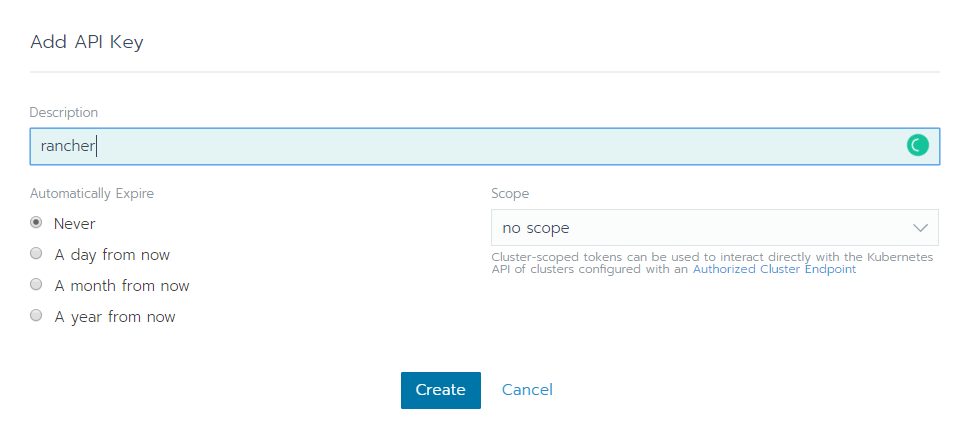
\includegraphics[width=\linewidth]{images/rancher-api-key.png}
\label{fig:rancherAPI}
\end{figure}

We'll then take the defined token and create the Rancher provider in our plan file \verb|provider.tf|:

\begin{lstlisting}[caption=Rancher Provider, frame=single, basicstyle=\ttfamily]
# Rancher
provider "rancher2" {
  api_url = var.rancher-url
  token_key = var.rancher-token
}
\end{lstlisting}

The code above is all the end-user credential and provider setup we'll need to create a Kubernetes cluster. On \verb|terraform init| the Rancher provider library will be downloaded and initialized. 

\subsection{Cloud Credentials}

It is good practice to keep the provider definitions separate from the main plan, so from here on, all example plan code will go into the main plan file, \verb|main.tf|. Also, from here on, the example plan code will be specific to deployment on Microsoft Azure, but you can easily adapt it for Amazon Web Services.

The first template we want to define is the cloud credentials. Regardless of the cloud provider, we need to provide some form of access credentials. On Microsoft Azure, this has to be done in the form of a service principal. These credentials could be created by the user, or better, be pre-provisioned by the IT organization.

In our Terraform plan, creating the credentials looks like this:

\begin{lstlisting}[caption=Cloud Credentials, frame=single, basicstyle=\ttfamily]
# Rancher cloud credentials
resource "rancher2_cloud_credential" "credential_az" {
  name = "Azure Credentials"
  azure_credential_config {
    client_id = var.az-client-id
    client_secret = var.az-client-secret
    subscription_id = var.az-subscription-id
  }
}
\end{lstlisting}

To create credentials we can also use the Rancher GUI with the same input fields:

\begin{figure}[H]
\centering
\caption {Cloud Credentials}
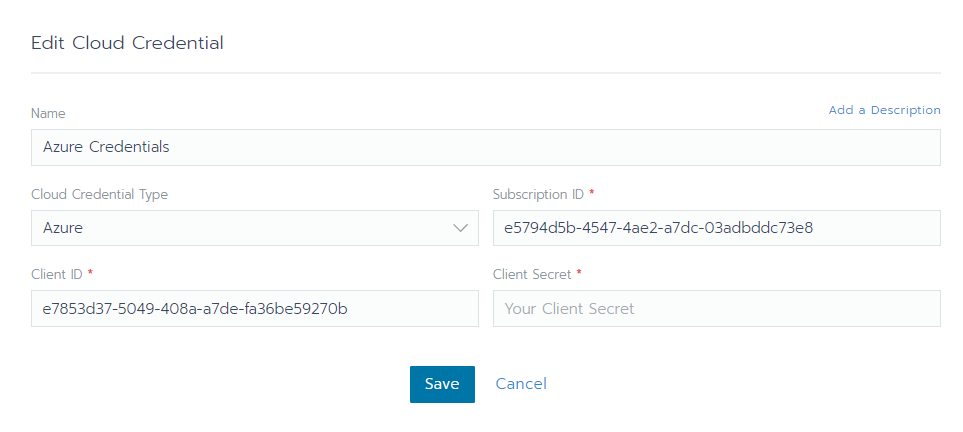
\includegraphics[width=\linewidth]{images/cloud-credentials.png}
\label{fig:cloudCredentials}
\end{figure}

\subsection{Node Templates}

As we've learned earlier, a Kubernetes cluster consists of one or more node pools, at least one for the control plane and one or more for the worker nodes. On a small installation, the control plane and the workers can be in the same node pool.

To create a node pool, we first need to define node templates in our plan:

\begin{lstlisting}[caption=Node Template, frame=single, basicstyle=\ttfamily]
# Rancher node template
resource "rancher2_node_template" "template_az" {
  name = "Azure Node Template"
  cloud_credential_id = rancher2_cloud_credential...id
  engine_install_url = var.dockerurl
  azure_config {
    disk_size = var.disksize
    image = var.image
    location = var.az-region
    managed_disks = true
    open_port = var.az-portlist
    resource_group = var.az-resource-group
    storage_type = var.az-storage-type
    size = var.type
  }
}
\end{lstlisting}

In a node template, we define size, OS image, and regional placement of the node. Depending on the future role, we can define them as small or as big as we need them, or define nodes with specialized hardware, such as GPUs, for machine-learning tasks.

We can make the same definition of node pools as above with the Rancher GUI:

\begin{figure}[H]
\centering
\caption {Node Template}
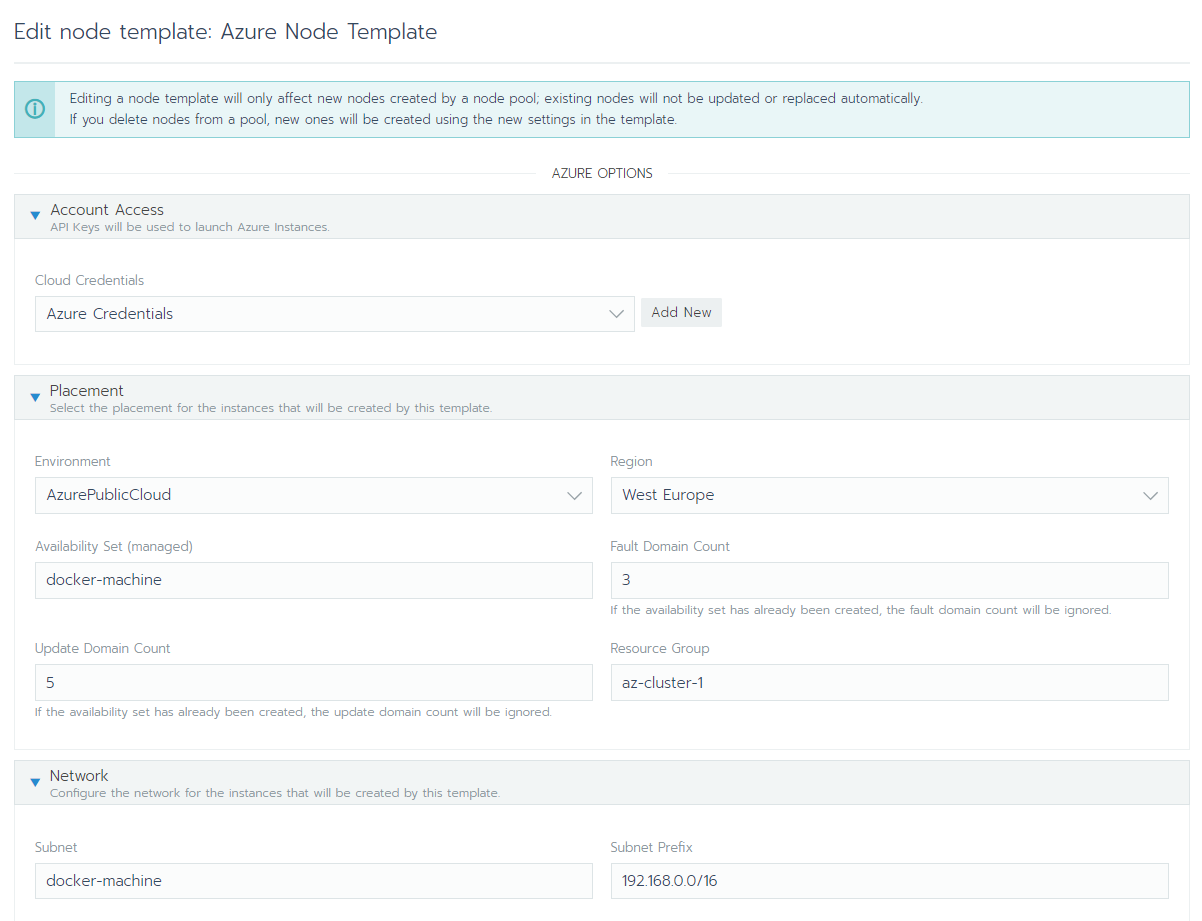
\includegraphics[width=\linewidth]{images/node-template.png}
\label{fig:nodeTemplate}
\end{figure}

The actual node pools will be created later; the template only defines their physical characteristics.

\subsection{Cluster Templates}

The third and final template that we are going to define is the template for the actual cluster.

\begin{lstlisting}[caption=Cluster Template, frame=single, basicstyle=\ttfamily]
# Rancher cluster template 
resource "rancher2_cluster_template" "template_az" {
  name = "Azure Cluster Template"
  template_revisions {
    name = "v1"
    default = true
    cluster_config {
      cluster_auth_endpoint {
        enabled = false
      }
      rke_config {
        kubernetes_version = var.k8version
        ignore_docker_version = false
        cloud_provider {
          name = "azure"
          azure_cloud_provider {
            aad_client_id = var.az-client-id
            aad_client_secret = var.az-client-secret
            subscription_id = var.az-subscription-id
            tenant_id = var.az-tenant-id
            resource_group = var.az-resource-group
          }
        }
      }
    }
  }
}
\end{lstlisting}

In this template, we define all the essential characteristics of our Kubernetes clusters that we want to enforce across the IT organization. For example, in the plan above, we do not allow users to bypass Rancher and access the Kubernetes clusters directly. This setting will give us a solid first line of defense against malicious attacks based on access credentials.

If you prefer the Rancher GUI, you can create cluster templates there, too:

\begin{figure}[H]
\centering
\caption {Cluster Template}
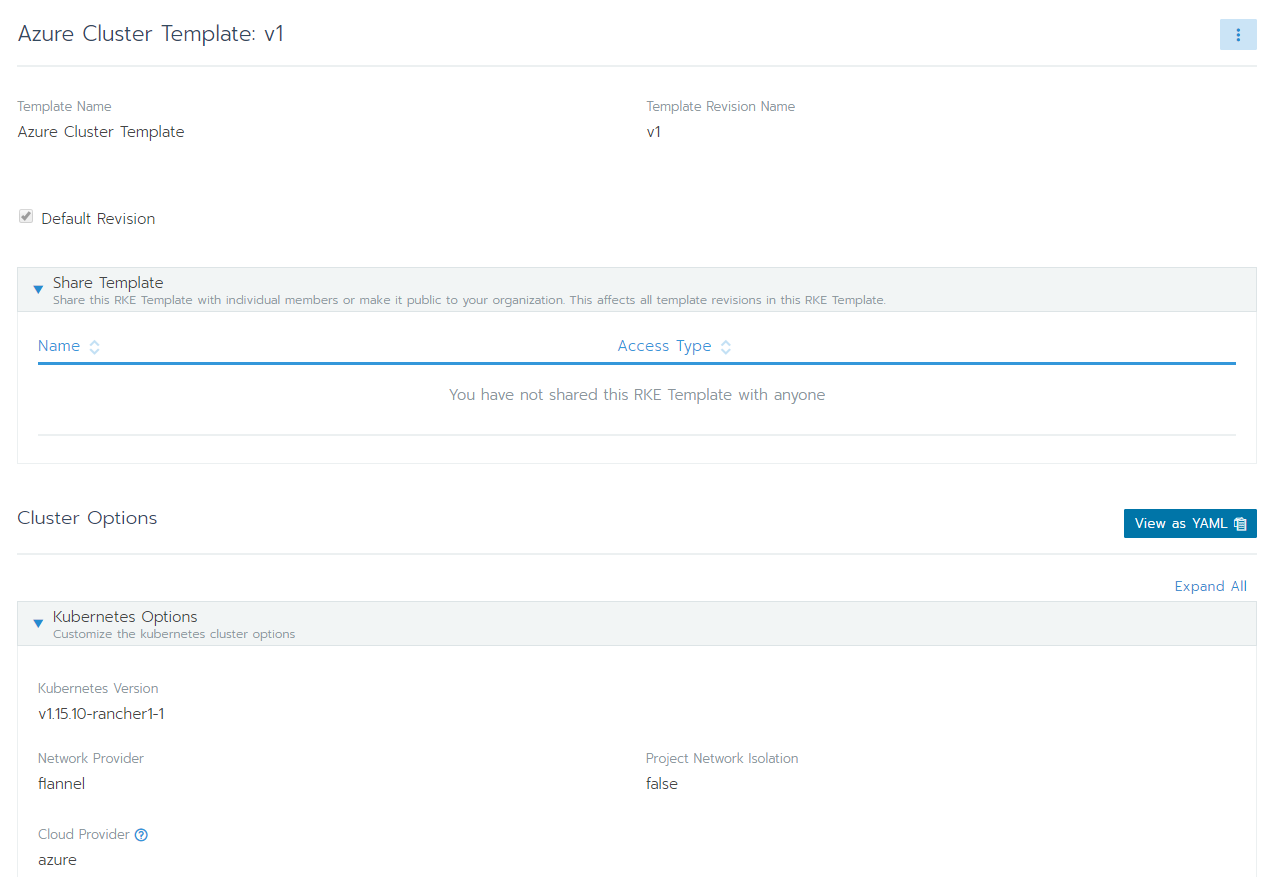
\includegraphics[width=\linewidth]{images/cluster-template.png}
\label{fig:clusterTemplate}
\end{figure}

\subsection{Kubernetes Cluster}

Now we have all the components together to build a Kubernetes cluster - credentials, node, and cluster templates. 

A fresh Kubernetes cluster is now only a few lines in our plan:

\begin{lstlisting}[caption=Kubernetes Cluster, frame=single, basicstyle=\ttfamily]
# Rancher cluster
resource "rancher2_cluster" "cluster_az" {
  name         = "az-${random_id.instance_id.hex}"
  description  = "Terraform"
  cluster_template_id = ...template_az.id
  cluster_template_revision_id = ...default_revision_id
  depends_on = [rancher2_cluster_template.template_az]
}
\end{lstlisting}

We give our cluster a name and a description and link it to the three templates we defined before. 

We also need at least one node pool in our plan:

\begin{lstlisting}[caption=Node Pool, frame=single, basicstyle=\ttfamily]
# Rancher node pool
resource "rancher2_node_pool" "nodepool_az" {
  cluster_id = rancher2_cluster.cluster_az.id
  name = "nodepool"
  hostname_prefix = "rke-${random_id.instance_id.hex}-"
  node_template_id = rancher2_node_template.template_az.id
  quantity = var.numnodes
  control_plane = true
  etcd = true
  worker = true
}
\end{lstlisting}

In this example, we define a single node pool with control plane and worker roles. Now we're done, and we can check the syntax of our plan files with \verb|terraform plan|, and then execute the plan with \verb|terraform apply|.

That's all that it takes!

In the Rancher GUI, creating a cluster is equally easy:

\begin{figure}[H]
\centering
\caption {Cluster Creation}
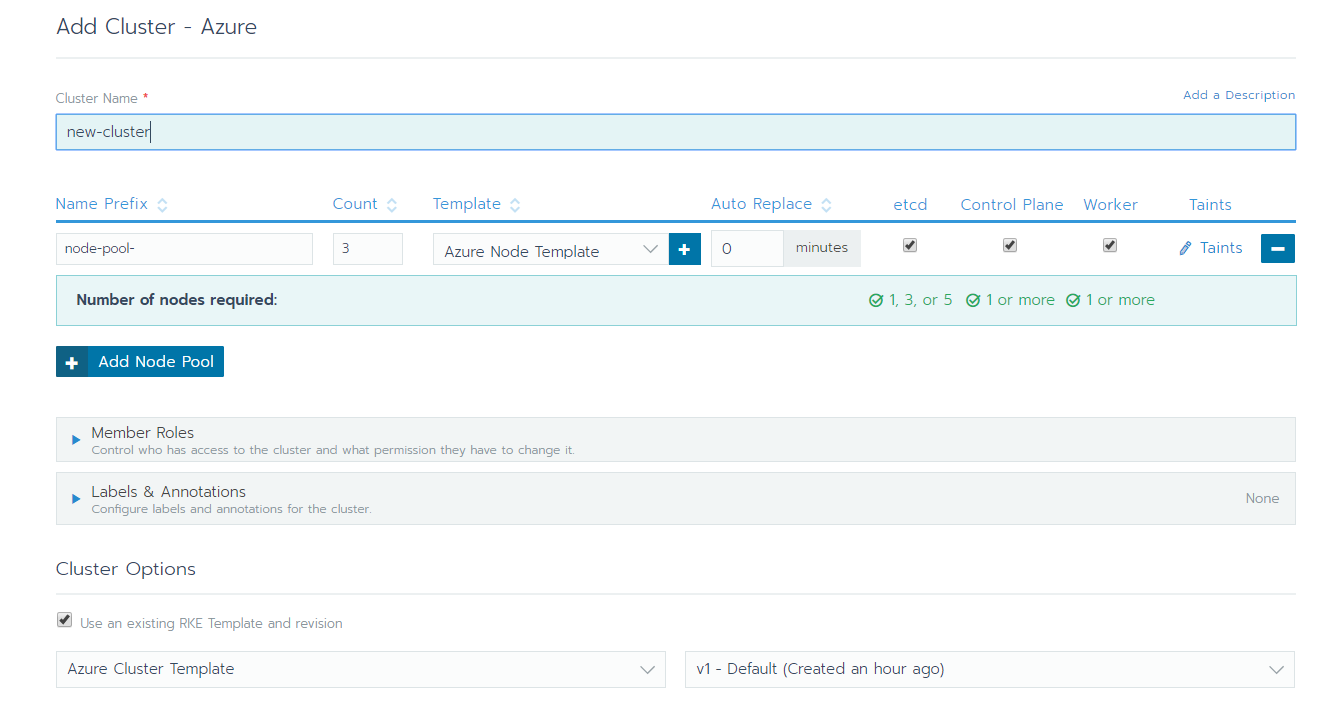
\includegraphics[width=\linewidth]{images/cluster-creation.png}
\label{fig:clusterCreation}
\end{figure}

With predefined templates, creating well-defined Kubernetes clusters is no longer a difficult task at all, and it does no longer require any in-depth knowledge of Kubernetes.

After successful creation, Rancher provides a convenient dashboard for the newly created cluster:

\begin{figure}[H]
\centering
\caption {Rancher Dashboard}
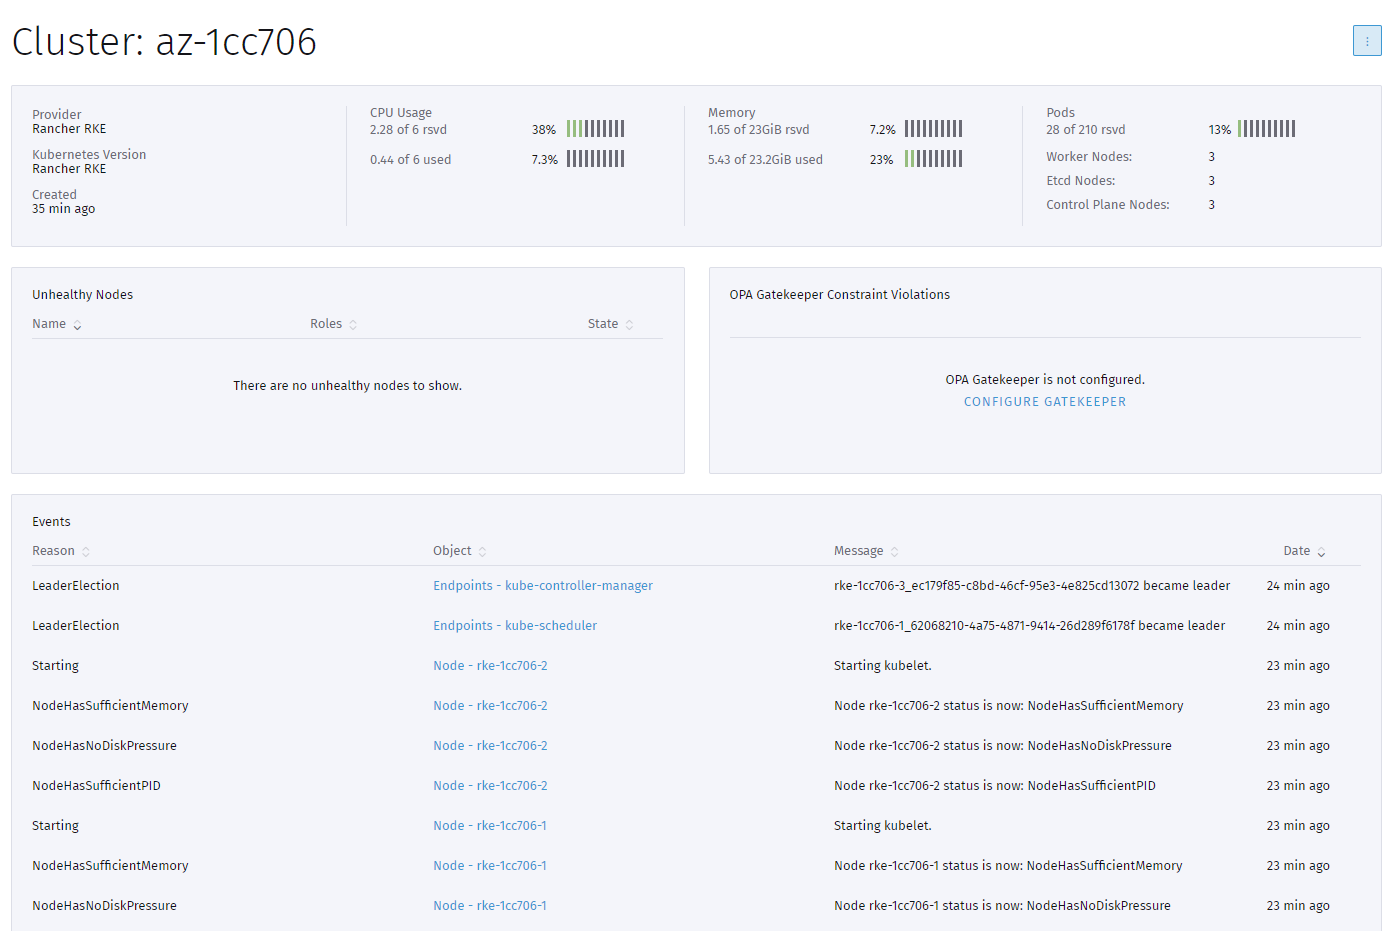
\includegraphics[width=\linewidth]{images/cluster-dashboard-new.png}
\label{fig:clusterOverview}
\end{figure}

This figure above shows the new Rancher dashboard layout, as introduced in March 2020 with Rancher 2.4.
